\documentclass[12pt]{article}
\usepackage[margin=1.2in]{geometry}
\usepackage{amsmath}
\usepackage{graphicx}
\begin{document}

\title{Plan for the Quantum computer demo}
\author{John Scott, Oliver Thomas}
\date

\maketitle

\section{Description for the demo}

We have built a 4 qubit prototype \textit{costing only \pounds10} and uses a rechargeable battery. We use LEDs to show the qubits and there are buttons for user input, we have also written some quantum algorithms which you can run and see what happens to the qubits as it runs. We would like to build a 16 qubit version, however we require more funds to pursue this.

\begin{figure}[h]
  \centering
    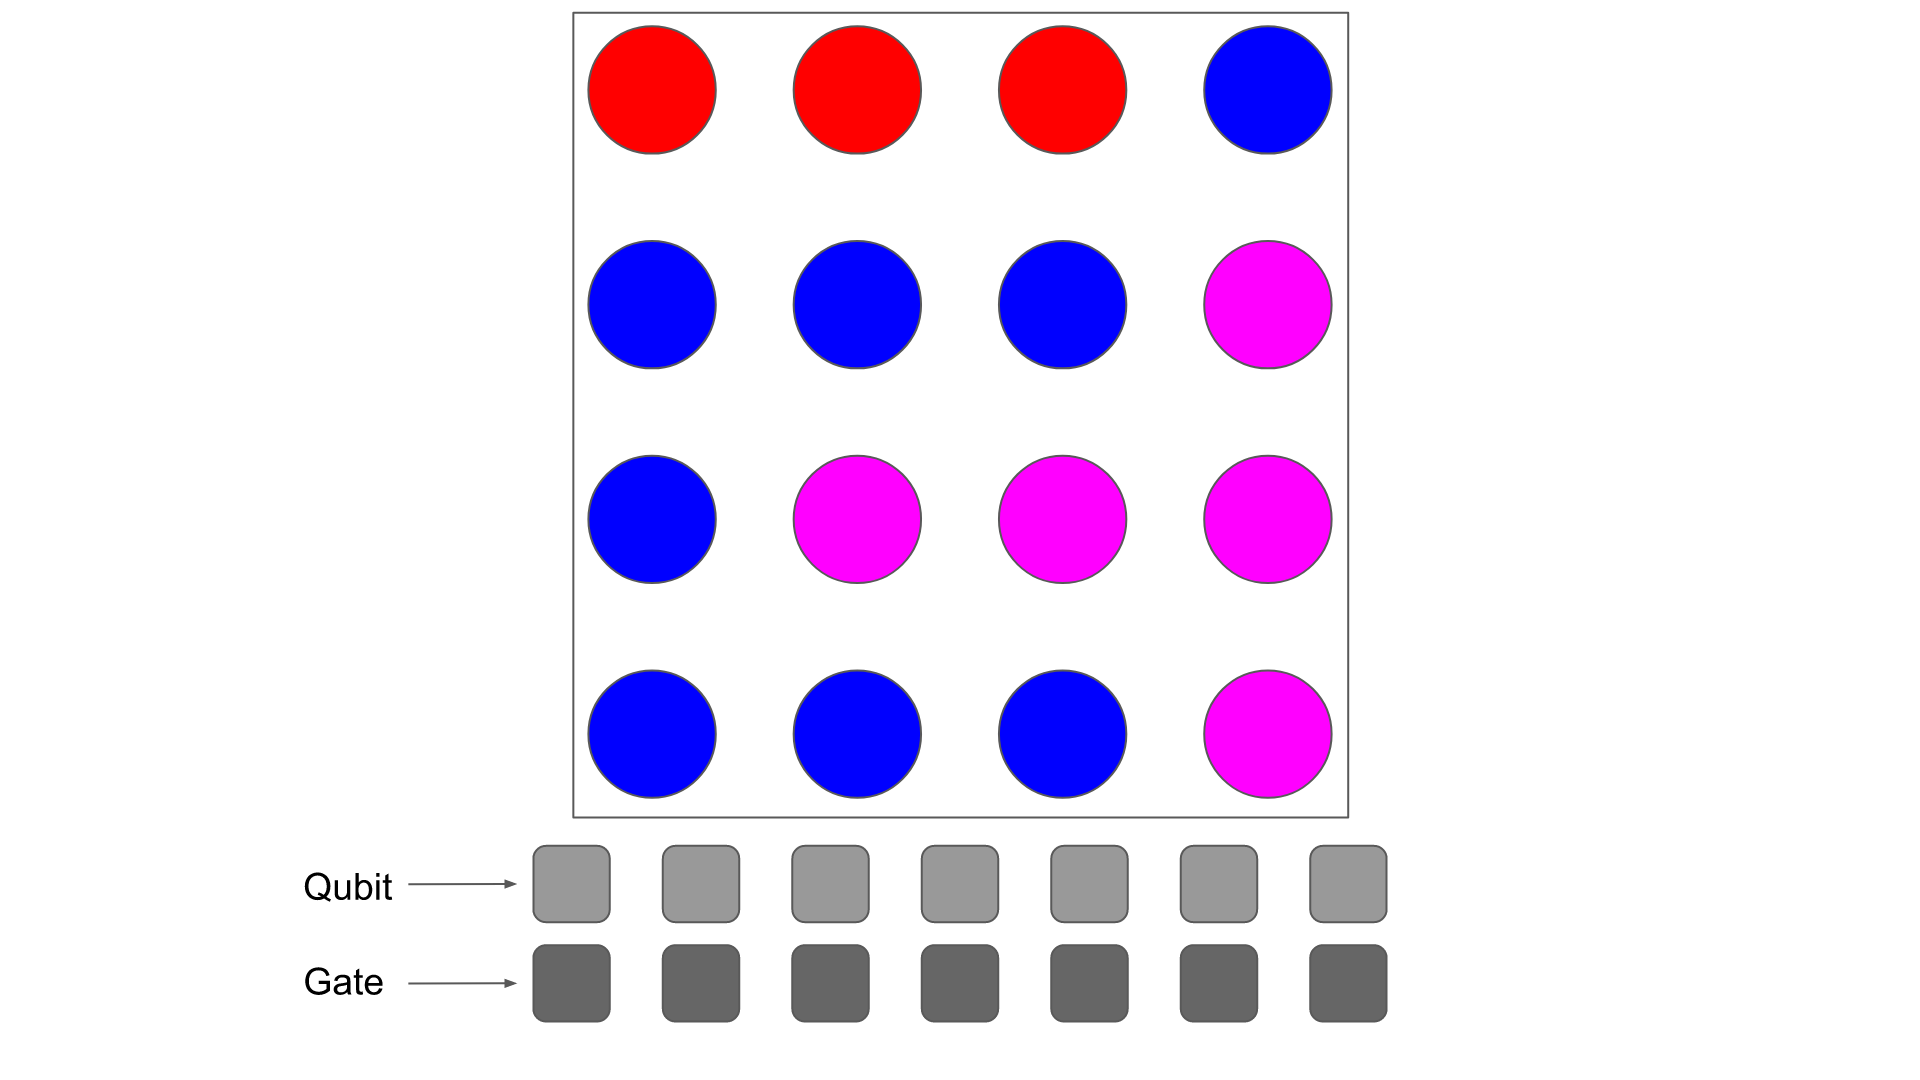
\includegraphics[width=0.8\textwidth]{qcomp.png}
    \caption{Artist's impression of the 16-qubit quantum computer. Qubits are
        denoted by circles with the colour representing their state. The buttons below
    control the device.}  
\end{figure}

\section{Things to be done}

\begin{itemize}
    \item Poster explaining the demo and what the different qubit colours mean 
    \item A list of quantum algorithms to be implemented
    \item Rules for a game, start out in certain pattern and have to use quantum gates to
        get to a target pattern
    \item QKD protocol across the grid of 16 qubits 
    \item Discussion on how to represent the qubits using Leds
    \item Ideas for how we should layout the qubit leds and button placements
    \item Building external housing and colour-scheme
\end{itemize}



\newpage 

\section{Part list}

\subsection{Necessary -- \pounds214.00}
\begin{itemize}
\item LEDs: \pounds1 each, \pounds16.00 in total for 16
\item LED drivers: \pounds0.72 each, \pounds5.76 for 8 chips
\item Buttons: \pounds1 each, \pounds20.00 in total for 20 buttons (may need bigger buttons later for the final demo)
\item Shift registers: \pounds0.32 each, \pounds1.60 for 5 chips
\item Transistors: \pounds0.12 each, \pounds6.00 for 50
\item Resistors: \pounds5.00
\item Breadboard and prototyping (reusable for other projects): \pounds50
\item Microcontroller (dsPIC33F): \pounds4.54
\item Memory chip: \pounds1.68 each, \pounds5.04
\item Final PCB: Under \pounds100.
\end{itemize}
\end{itemize}

\subsection{Optional -- \pounds110.00}

\begin{itemize}
\item Development board: \pounds110.00

\end{itemize}
\end{itemize}



\end{document}



